% Generated by Sphinx.
\def\sphinxdocclass{report}
\documentclass[letterpaper,10pt,english]{sphinxmanual}
\usepackage[utf8]{inputenc}
\DeclareUnicodeCharacter{00A0}{\nobreakspace}
\usepackage[T1]{fontenc}
\usepackage{babel}
\usepackage{times}
\usepackage[Bjarne]{fncychap}
\usepackage{longtable}
\usepackage{sphinx}
\usepackage{multirow}


\title{pyPLUTO Documentation}
\date{May 04, 2012}
\release{1.0}
\author{Bhargav Vaidya , Denis Stepanovs}
\newcommand{\sphinxlogo}{}
\renewcommand{\releasename}{Release}
\makeindex

\makeatletter
\def\PYG@reset{\let\PYG@it=\relax \let\PYG@bf=\relax%
    \let\PYG@ul=\relax \let\PYG@tc=\relax%
    \let\PYG@bc=\relax \let\PYG@ff=\relax}
\def\PYG@tok#1{\csname PYG@tok@#1\endcsname}
\def\PYG@toks#1+{\ifx\relax#1\empty\else%
    \PYG@tok{#1}\expandafter\PYG@toks\fi}
\def\PYG@do#1{\PYG@bc{\PYG@tc{\PYG@ul{%
    \PYG@it{\PYG@bf{\PYG@ff{#1}}}}}}}
\def\PYG#1#2{\PYG@reset\PYG@toks#1+\relax+\PYG@do{#2}}

\def\PYG@tok@gd{\def\PYG@tc##1{\textcolor[rgb]{0.63,0.00,0.00}{##1}}}
\def\PYG@tok@gu{\let\PYG@bf=\textbf\def\PYG@tc##1{\textcolor[rgb]{0.50,0.00,0.50}{##1}}}
\def\PYG@tok@gt{\def\PYG@tc##1{\textcolor[rgb]{0.00,0.25,0.82}{##1}}}
\def\PYG@tok@gs{\let\PYG@bf=\textbf}
\def\PYG@tok@gr{\def\PYG@tc##1{\textcolor[rgb]{1.00,0.00,0.00}{##1}}}
\def\PYG@tok@cm{\let\PYG@it=\textit\def\PYG@tc##1{\textcolor[rgb]{0.25,0.50,0.56}{##1}}}
\def\PYG@tok@vg{\def\PYG@tc##1{\textcolor[rgb]{0.73,0.38,0.84}{##1}}}
\def\PYG@tok@m{\def\PYG@tc##1{\textcolor[rgb]{0.13,0.50,0.31}{##1}}}
\def\PYG@tok@mh{\def\PYG@tc##1{\textcolor[rgb]{0.13,0.50,0.31}{##1}}}
\def\PYG@tok@cs{\def\PYG@tc##1{\textcolor[rgb]{0.25,0.50,0.56}{##1}}\def\PYG@bc##1{\colorbox[rgb]{1.00,0.94,0.94}{##1}}}
\def\PYG@tok@ge{\let\PYG@it=\textit}
\def\PYG@tok@vc{\def\PYG@tc##1{\textcolor[rgb]{0.73,0.38,0.84}{##1}}}
\def\PYG@tok@il{\def\PYG@tc##1{\textcolor[rgb]{0.13,0.50,0.31}{##1}}}
\def\PYG@tok@go{\def\PYG@tc##1{\textcolor[rgb]{0.19,0.19,0.19}{##1}}}
\def\PYG@tok@cp{\def\PYG@tc##1{\textcolor[rgb]{0.00,0.44,0.13}{##1}}}
\def\PYG@tok@gi{\def\PYG@tc##1{\textcolor[rgb]{0.00,0.63,0.00}{##1}}}
\def\PYG@tok@gh{\let\PYG@bf=\textbf\def\PYG@tc##1{\textcolor[rgb]{0.00,0.00,0.50}{##1}}}
\def\PYG@tok@ni{\let\PYG@bf=\textbf\def\PYG@tc##1{\textcolor[rgb]{0.84,0.33,0.22}{##1}}}
\def\PYG@tok@nl{\let\PYG@bf=\textbf\def\PYG@tc##1{\textcolor[rgb]{0.00,0.13,0.44}{##1}}}
\def\PYG@tok@nn{\let\PYG@bf=\textbf\def\PYG@tc##1{\textcolor[rgb]{0.05,0.52,0.71}{##1}}}
\def\PYG@tok@no{\def\PYG@tc##1{\textcolor[rgb]{0.38,0.68,0.84}{##1}}}
\def\PYG@tok@na{\def\PYG@tc##1{\textcolor[rgb]{0.25,0.44,0.63}{##1}}}
\def\PYG@tok@nb{\def\PYG@tc##1{\textcolor[rgb]{0.00,0.44,0.13}{##1}}}
\def\PYG@tok@nc{\let\PYG@bf=\textbf\def\PYG@tc##1{\textcolor[rgb]{0.05,0.52,0.71}{##1}}}
\def\PYG@tok@nd{\let\PYG@bf=\textbf\def\PYG@tc##1{\textcolor[rgb]{0.33,0.33,0.33}{##1}}}
\def\PYG@tok@ne{\def\PYG@tc##1{\textcolor[rgb]{0.00,0.44,0.13}{##1}}}
\def\PYG@tok@nf{\def\PYG@tc##1{\textcolor[rgb]{0.02,0.16,0.49}{##1}}}
\def\PYG@tok@si{\let\PYG@it=\textit\def\PYG@tc##1{\textcolor[rgb]{0.44,0.63,0.82}{##1}}}
\def\PYG@tok@s2{\def\PYG@tc##1{\textcolor[rgb]{0.25,0.44,0.63}{##1}}}
\def\PYG@tok@vi{\def\PYG@tc##1{\textcolor[rgb]{0.73,0.38,0.84}{##1}}}
\def\PYG@tok@nt{\let\PYG@bf=\textbf\def\PYG@tc##1{\textcolor[rgb]{0.02,0.16,0.45}{##1}}}
\def\PYG@tok@nv{\def\PYG@tc##1{\textcolor[rgb]{0.73,0.38,0.84}{##1}}}
\def\PYG@tok@s1{\def\PYG@tc##1{\textcolor[rgb]{0.25,0.44,0.63}{##1}}}
\def\PYG@tok@gp{\let\PYG@bf=\textbf\def\PYG@tc##1{\textcolor[rgb]{0.78,0.36,0.04}{##1}}}
\def\PYG@tok@sh{\def\PYG@tc##1{\textcolor[rgb]{0.25,0.44,0.63}{##1}}}
\def\PYG@tok@ow{\let\PYG@bf=\textbf\def\PYG@tc##1{\textcolor[rgb]{0.00,0.44,0.13}{##1}}}
\def\PYG@tok@sx{\def\PYG@tc##1{\textcolor[rgb]{0.78,0.36,0.04}{##1}}}
\def\PYG@tok@bp{\def\PYG@tc##1{\textcolor[rgb]{0.00,0.44,0.13}{##1}}}
\def\PYG@tok@c1{\let\PYG@it=\textit\def\PYG@tc##1{\textcolor[rgb]{0.25,0.50,0.56}{##1}}}
\def\PYG@tok@kc{\let\PYG@bf=\textbf\def\PYG@tc##1{\textcolor[rgb]{0.00,0.44,0.13}{##1}}}
\def\PYG@tok@c{\let\PYG@it=\textit\def\PYG@tc##1{\textcolor[rgb]{0.25,0.50,0.56}{##1}}}
\def\PYG@tok@mf{\def\PYG@tc##1{\textcolor[rgb]{0.13,0.50,0.31}{##1}}}
\def\PYG@tok@err{\def\PYG@bc##1{\fcolorbox[rgb]{1.00,0.00,0.00}{1,1,1}{##1}}}
\def\PYG@tok@kd{\let\PYG@bf=\textbf\def\PYG@tc##1{\textcolor[rgb]{0.00,0.44,0.13}{##1}}}
\def\PYG@tok@ss{\def\PYG@tc##1{\textcolor[rgb]{0.32,0.47,0.09}{##1}}}
\def\PYG@tok@sr{\def\PYG@tc##1{\textcolor[rgb]{0.14,0.33,0.53}{##1}}}
\def\PYG@tok@mo{\def\PYG@tc##1{\textcolor[rgb]{0.13,0.50,0.31}{##1}}}
\def\PYG@tok@mi{\def\PYG@tc##1{\textcolor[rgb]{0.13,0.50,0.31}{##1}}}
\def\PYG@tok@kn{\let\PYG@bf=\textbf\def\PYG@tc##1{\textcolor[rgb]{0.00,0.44,0.13}{##1}}}
\def\PYG@tok@o{\def\PYG@tc##1{\textcolor[rgb]{0.40,0.40,0.40}{##1}}}
\def\PYG@tok@kr{\let\PYG@bf=\textbf\def\PYG@tc##1{\textcolor[rgb]{0.00,0.44,0.13}{##1}}}
\def\PYG@tok@s{\def\PYG@tc##1{\textcolor[rgb]{0.25,0.44,0.63}{##1}}}
\def\PYG@tok@kp{\def\PYG@tc##1{\textcolor[rgb]{0.00,0.44,0.13}{##1}}}
\def\PYG@tok@w{\def\PYG@tc##1{\textcolor[rgb]{0.73,0.73,0.73}{##1}}}
\def\PYG@tok@kt{\def\PYG@tc##1{\textcolor[rgb]{0.56,0.13,0.00}{##1}}}
\def\PYG@tok@sc{\def\PYG@tc##1{\textcolor[rgb]{0.25,0.44,0.63}{##1}}}
\def\PYG@tok@sb{\def\PYG@tc##1{\textcolor[rgb]{0.25,0.44,0.63}{##1}}}
\def\PYG@tok@k{\let\PYG@bf=\textbf\def\PYG@tc##1{\textcolor[rgb]{0.00,0.44,0.13}{##1}}}
\def\PYG@tok@se{\let\PYG@bf=\textbf\def\PYG@tc##1{\textcolor[rgb]{0.25,0.44,0.63}{##1}}}
\def\PYG@tok@sd{\let\PYG@it=\textit\def\PYG@tc##1{\textcolor[rgb]{0.25,0.44,0.63}{##1}}}

\def\PYGZbs{\char`\\}
\def\PYGZus{\char`\_}
\def\PYGZob{\char`\{}
\def\PYGZcb{\char`\}}
\def\PYGZca{\char`\^}
\def\PYGZsh{\char`\#}
\def\PYGZpc{\char`\%}
\def\PYGZdl{\char`\$}
\def\PYGZti{\char`\~}
% for compatibility with earlier versions
\def\PYGZat{@}
\def\PYGZlb{[}
\def\PYGZrb{]}
\makeatother

\begin{document}

\maketitle
\tableofcontents
\phantomsection\label{index::doc}



\chapter{Information}
\label{index:information}\label{index:welcome-to-pypluto-s-documentation}
This is the documentation for pyPLUTO code.
This is created using a cool software named Sphinx.
\begin{quote}\begin{description}
\item[{Author}] \leavevmode
Bhargav Vaidya (b.vaidya at leeds.ac.uk) and Denis Stepanovs (stepanovs at mpia.de)

\item[{Release}] \leavevmode
1.0

\item[{Date}] \leavevmode
May 04, 2012

\end{description}\end{quote}


\section{Installation}
\label{install:installation}\label{install::doc}
After ensuring that all of the above pre-requisites are working and
installed the user can download  pyPLUTO-1.zip from \href{http://www.ast.leeds.ac.uk/~phybva/Bhargav\_Vaidya/Simulations.html}{here}.

The code can be installed using a standard procedure. This can be done by following steps:
\begin{enumerate}
\item {} 
\textbf{Global Install}

\end{enumerate}

The Python version from the EPD version by default creates a PYTHONPATH. If no option is chosen for preferred path
then in that case the code will be installed in that default path.  This might require the user to have access to the root password:
\begin{itemize}
\item {} 
Unzip the source code : \code{unzip pyPLUTO-1.0.zip}

\item {} 
Enter into the directory : \code{cd pyPLUTO-1.0}

\item {} 
Install the code in the default path : \code{python setup.py install}

\end{itemize}
\begin{enumerate}
\setcounter{enumi}{1}
\item {} 
\textbf{Local Install}

\end{enumerate}

The best practice is to create your own PYTHONPATH and do a local install in the following way:
\begin{itemize}
\item {} 
Create a directory where to store this module : \code{mkdir MyPython\_Modules}

\item {} 
Unzip the source code : \code{unzip pyPLUTO-1.0.zip}

\item {} 
Enter into the directory : \code{cd pyPLUTO-1.0}

\item {} 
Install the code in the directory created : \code{python setup.py install -{-}prefix=\textless{}path to MyPython\_Modules\textgreater{}}

\item {} 
Then append the following in your .bashrc : \code{export PYTHONPATH = \$HOME/MyPython\_Modules/lib/python\textless{}ver\textgreater{}/site-packages}

\end{itemize}

where \textless{}ver\textgreater{} is the python version which the user have used to install the package.

After the successful installation, the user can start using GUI application by appending the \textless{}path to GUI\_pyPLUTO.py\textgreater{} into their PATH.


\section{Loading the Data}
\label{pload:loading-the-data}\label{pload::doc}\index{pload (class in pyPLUTO)}

\begin{fulllineitems}
\phantomsection\label{pload:pyPLUTO.pload}\pysiglinewithargsret{\strong{class }\code{pyPLUTO.}\bfcode{pload}}{\emph{ns}, \emph{w\_dir=None}}{}
This Class has all the routines loading the data from the
binary files output from PLUTO Simulations. Assign an object
when the data is loaded for some \emph{ns}.

\emph{Usage}:

\code{import pyPLUTO as pp}

\code{wdir = '/path/to/the data files/'}

\code{D = pp.pload(1,w\_dir=wdir)}

Now D is the pyPLUTO.pload object having all the relevant information
of the corresponding data file - data.0001.dbl.

It has the following attributes --
\index{data() (pyPLUTO.pload method)}

\begin{fulllineitems}
\phantomsection\label{pload:pyPLUTO.pload.data}\pysiglinewithargsret{\bfcode{data}}{}{}
This method loads the data from the file name ``data.ns.dbl'' or ``varname.ns.dbl''.

\end{fulllineitems}

\index{geometry() (pyPLUTO.pload method)}

\begin{fulllineitems}
\phantomsection\label{pload:pyPLUTO.pload.geometry}\pysiglinewithargsret{\bfcode{geometry}}{}{}
This method has the geometry information of the problem considered.

\end{fulllineitems}

\index{get\_varinfo() (pyPLUTO.pload method)}

\begin{fulllineitems}
\phantomsection\label{pload:pyPLUTO.pload.get_varinfo}\pysiglinewithargsret{\bfcode{get\_varinfo}}{}{}
This method reads the dbl.out and stores the information in a dictionary.

\emph{Keyword Arguments}:

fltype -- returns the filetype of storing data (single\_file or multiple\_file)

nvar -- Number of variables

allvars -- A list of variables names. Each of the variable name will be the attributes to the pyPLUTO.pload object.

\end{fulllineitems}

\index{grid() (pyPLUTO.pload method)}

\begin{fulllineitems}
\phantomsection\label{pload:pyPLUTO.pload.grid}\pysiglinewithargsret{\bfcode{grid}}{}{}
This method returns the necessary grid information in form a dictionary.

\emph{Keyword Arguments}:

n1 -- number of grid cells in x1 direction

n2 -- number of grid cells in x2 direction

n3 -- number of grid cells in x3 direction

x1 -- Array x1

x2 - Array x2

x3 - Array x3

dx1 - Array dx1

dx2 - Array dx2

dx3 - Array dx3

\end{fulllineitems}

\index{time\_info() (pyPLUTO.pload method)}

\begin{fulllineitems}
\phantomsection\label{pload:pyPLUTO.pload.time_info}\pysiglinewithargsret{\bfcode{time\_info}}{}{}
This method returns a dictionary that has the time information for the
step ns.

\emph{Keyword Arguments}:

time -- Gets the simulation time at step ns.

dt -- Get the time step dt for step ns.

Nstep -- Get the value of nstep for the step ns.

\end{fulllineitems}


\end{fulllineitems}



\section{Viewing the Data}
\label{image:viewing-the-data}\label{image::doc}\index{Image (class in pyPLUTO)}

\begin{fulllineitems}
\phantomsection\label{image:pyPLUTO.Image}\pysigline{\strong{class }\code{pyPLUTO.}\bfcode{Image}}
This Class has all the routines for the imaging the data
and plotting various contours and fieldlines on these images.
CALLED AFTER pyPLUTO.pload object is defined
\index{field\_interp() (pyPLUTO.Image method)}

\begin{fulllineitems}
\phantomsection\label{image:pyPLUTO.Image.field_interp}\pysiglinewithargsret{\bfcode{field\_interp}}{\emph{var1}, \emph{var2}, \emph{x}, \emph{y}, \emph{dx}, \emph{dy}, \emph{xp}, \emph{yp}}{}
This method interpolates value of vector fields (var1 and var2) on field points (xp and yp).
The field points are obtained from the method field\_line.
\begin{description}
\item[{\emph{Arguments}:}] \leavevmode
var1 -- 2D Vector field in X direction

var2 -- 2D Vector field in Y direction

x -- 1D X array

y -- 1D Y array

dx -- 1D grid spacing array in X direction

dy -- 1D grid spacing array in Y direction

xp -- field point in X direction

yp -- field point in Y direction

\end{description}

\end{fulllineitems}

\index{field\_line() (pyPLUTO.Image method)}

\begin{fulllineitems}
\phantomsection\label{image:pyPLUTO.Image.field_line}\pysiglinewithargsret{\bfcode{field\_line}}{\emph{var1}, \emph{var2}, \emph{x}, \emph{y}, \emph{dx}, \emph{dy}, \emph{x0}, \emph{y0}}{}
This method is used to obtain field lines (same as fieldline.pro in PLUTO IDL tools).
\begin{description}
\item[{\emph{Arguments}:}] \leavevmode
var1 -- 2D Vector field in X direction

var2 -- 2D Vector field in Y direction

x -- 1D X array

y -- 1D Y array

dx -- 1D grid spacing array in X direction

dy -- 1D grid spacing array in Y direction

x0 -- foot point of the field line in X direction

y0 -- foot point of the field line in Y direction

\end{description}

\end{fulllineitems}

\index{getSphData() (pyPLUTO.Image method)}

\begin{fulllineitems}
\phantomsection\label{image:pyPLUTO.Image.getSphData}\pysiglinewithargsret{\bfcode{getSphData}}{\emph{Data}, \emph{w\_dir=None}, \emph{**kwargs}}{}
This method transforms the vector and scalar  fields from Spherical co-ordinates to Cylindrical.

\emph{Arguments}:
\begin{quote}

Data -- puPLUTO.pload object

w\_dir -- /path/to/the/working/directory/
\end{quote}

\emph{Keywords}:
\begin{quote}

rphi -- {[}Default{]} is set to False implies that the r-theta plane is transformed. If set True then the r-phi plane is transformed.

x2cut -- Applicable for 3D data and it determines the co-ordinate of the x2 plane while r-phi is set to True.

x3cut -- Applicable for 3D data and it determines the co-ordinate of the x3 plane while r-phi is set to False.
\end{quote}

\end{fulllineitems}

\index{myfieldlines() (pyPLUTO.Image method)}

\begin{fulllineitems}
\phantomsection\label{image:pyPLUTO.Image.myfieldlines}\pysiglinewithargsret{\bfcode{myfieldlines}}{\emph{Data}, \emph{x0arr}, \emph{y0arr}, \emph{stream=False}, \emph{**kwargs}}{}
This method overplots the magnetic field lines at the footpoints given by (x0arr{[}i{]},y0arr{[}i{]}).

\emph{Arguments}:
\begin{quote}

Data -- pyPLUTO.pload object

x0arr -- array of x co-ordinates of the footpoints

y0arr -- array of y co-ordinates of the footpoints

stream -- keyword for two different ways of calculating the field lines.
\begin{quote}

True -- plots contours of rAphi (needs to store vector potential)

False -- plots the fieldlines obtained from the field\_line routine. (Default option)
\end{quote}
\end{quote}

\emph{Keywords}:
\begin{quote}

colors -- A list of matplotlib colors to represent the lines. The length of this list should be same as that of x0arr.

lw -- Integer value that determines the linewidth of each line.

ls -- Determines the linestyle of each line.
\end{quote}

\end{fulllineitems}

\index{pldisplay() (pyPLUTO.Image method)}

\begin{fulllineitems}
\phantomsection\label{image:pyPLUTO.Image.pldisplay}\pysiglinewithargsret{\bfcode{pldisplay}}{\emph{var}, \emph{**kwargs}}{}
This method allows the user to display a 2D data using the matplotlib's pcolormesh.

\emph{Arguments}:
\begin{quote}

var -- 2D array that needs to be displayed.
\end{quote}

\emph{Keywords}:
\begin{quote}

x1 -- The `x' array

x2 -- The `y' array

vmin -- The minimum value of the 2D array (Default : min(var))

vmax -- The maximum value of the 2D array (Default : max(var))

title -- Sets the title of the image.

label1 -- Sets the X Label (Default: `XLabel')

label2 -- Sets the Y Label (Default: `YLabel')
\begin{description}
\item[{cbar -- Its a tuple to set the colorbar on or off. }] \leavevmode
cbar = (True,'vertical') -- Displays a vertical colorbar

cbar = (True,'horizontal') -- Displays a horizontal colorbar

cbar = (False,'`) -- Displays no colorbar.

\end{description}
\end{quote}

\emph{Usage}:
\begin{quote}

\code{import pyPLUTO as pp}

\code{wdir = '/path/to/the data files/'}

\code{D = pp.pload(1,w\_dir=wdir)}

\code{I = pp.Image()}

\code{f1 = figure()}

\code{ax1 = f1.add\_subplot(111)}

\code{I.pldisplay(D.v2,x1=D.x1,x2=D.x2,cbar=(True,'vertical'),title='Velocity',label1='Radius',label2='Height')}
\end{quote}

\end{fulllineitems}

\index{pltSphData() (pyPLUTO.Image method)}

\begin{fulllineitems}
\phantomsection\label{image:pyPLUTO.Image.pltSphData}\pysiglinewithargsret{\bfcode{pltSphData}}{\emph{Data}, \emph{w\_dir=None}, \emph{**kwargs}}{}
This method plots the transformed data obtained from getSphData using the matplotlib's imshow

\emph{Arguments}:
\begin{quote}

Data -- pyPLUTO.pload object

w\_dir -- /path/to/the/working/directory/
\end{quote}

\emph{Keywords}:
\begin{quote}

plvar -- A string which represents the plot variable.
\end{quote}

\end{fulllineitems}


\end{fulllineitems}



\section{Additional tools}
\label{tools:additional-tools}\label{tools::doc}\index{Tools (class in pyPLUTO)}

\begin{fulllineitems}
\phantomsection\label{tools:pyPLUTO.Tools}\pysigline{\strong{class }\code{pyPLUTO.}\bfcode{Tools}}
This Class has all the functions doing basic mathematical
operations to the vector or scalar fields.
It is called after pyPLUTO.pload object is defined.
\index{Div() (pyPLUTO.Tools method)}

\begin{fulllineitems}
\phantomsection\label{tools:pyPLUTO.Tools.Div}\pysiglinewithargsret{\bfcode{Div}}{\emph{u1}, \emph{u2}, \emph{x1}, \emph{x2}, \emph{dx1}, \emph{dx2}, \emph{geometry=None}}{}
This method calculates the divergence of the 2D vector fields u1 and u2. It requires the vectors x1 and x2 with their respective grid spacings dx1 and dx2.

The keyword \emph{geometry} is by default set to `cartesian'. It can be set to eitherone of the following : \emph{cartesian}, \emph{cylindrical}, \emph{spherical} or \emph{polar}. To calculate the divergence of the vector fields, respective geometric corrections are taken into account based on the value of this keyword.

\end{fulllineitems}

\index{Grad() (pyPLUTO.Tools method)}

\begin{fulllineitems}
\phantomsection\label{tools:pyPLUTO.Tools.Grad}\pysiglinewithargsret{\bfcode{Grad}}{\emph{phi}, \emph{x1}, \emph{x2}, \emph{dx1}, \emph{dx2}, \emph{polar=False}}{}
This method calculates the gradient of the 2D scalar phi. It requires the vectors x1 and x2 with their respective grid spacings dx1 and dx2.

The keyword \emph{polar} is by default set to False, when set True respective geometric corrections are taken into account for calculating the gradient.

\end{fulllineitems}

\index{RTh2Cyl() (pyPLUTO.Tools method)}

\begin{fulllineitems}
\phantomsection\label{tools:pyPLUTO.Tools.RTh2Cyl}\pysiglinewithargsret{\bfcode{RTh2Cyl}}{\emph{R}, \emph{Th}, \emph{X1}, \emph{X2}}{}
Transforms vector (X1,X2) given in spherical coordinates to cylindrical. 
X1 and X2 could correspond to Br and Bth, R and Th - matrices with sph. coordinates
The result is (Y1,Y2) which correspond to vector in cylindrical coords (Br,Bz)

\end{fulllineitems}

\index{congrid() (pyPLUTO.Tools method)}

\begin{fulllineitems}
\phantomsection\label{tools:pyPLUTO.Tools.congrid}\pysiglinewithargsret{\bfcode{congrid}}{\emph{a}, \emph{newdims}, \emph{method='linear'}, \emph{centre=False}, \emph{minusone=False}}{}
Arbitrary resampling of source array to new dimension sizes.
Currently only supports maintaining the same number of dimensions.
To use 1-D arrays, first promote them to shape (x,1).

Uses the same parameters and creates the same co-ordinate lookup points
as IDL''s congrid routine, which apparently originally came from a VAX/VMS
routine of the same name.

method:

neighbour - closest value from original data
\begin{description}
\item[{nearest and linear - uses n x 1-D interpolations using}] \leavevmode
scipy.interpolate.interp1d

\end{description}

(see Numerical Recipes for validity of use of n 1-D interpolations)

spline - uses ndimage.map\_coordinates

centre:

True - interpolation points are at the centres of the bins

False - points are at the front edge of the bin

minusone:

For example- inarray.shape = (i,j) \& new dimensions = (x,y)

False - inarray is resampled by factors of (i/x) * (j/y)

True - inarray is resampled by(i-1)/(x-1) * (j-1)/(y-1)

This prevents extrapolation one element beyond bounds of input array.

\end{fulllineitems}

\index{deriv() (pyPLUTO.Tools method)}

\begin{fulllineitems}
\phantomsection\label{tools:pyPLUTO.Tools.deriv}\pysiglinewithargsret{\bfcode{deriv}}{\emph{Y}, \emph{X=None}}{}
Calculates the derivative of Y with respect to X.

Keywords:
Y : 1-D array to be differentiated.
X : 1-D array with len(X) = len(Y).

If X is not specified then by default X is chosen to be an equally spaced array having same number of elements
as Y.

\end{fulllineitems}

\index{getUniformGrid() (pyPLUTO.Tools method)}

\begin{fulllineitems}
\phantomsection\label{tools:pyPLUTO.Tools.getUniformGrid}\pysiglinewithargsret{\bfcode{getUniformGrid}}{\emph{r}, \emph{th}, \emph{rho}, \emph{Nr}, \emph{Nth}}{}
Transforms data with non-uniform axes (stretched) into uniform.
r, th - grids, rho(r,th) - data, Nr and Nth - sizes of new (uniform) grid

\end{fulllineitems}

\index{myInterpol() (pyPLUTO.Tools method)}

\begin{fulllineitems}
\phantomsection\label{tools:pyPLUTO.Tools.myInterpol}\pysiglinewithargsret{\bfcode{myInterpol}}{\emph{RR}, \emph{N}}{}
Interpolates vector RR to N-grids. Returns RRi-interpolated vector 
and NNi - grid of

\end{fulllineitems}

\index{sph2cyl() (pyPLUTO.Tools method)}

\begin{fulllineitems}
\phantomsection\label{tools:pyPLUTO.Tools.sph2cyl}\pysiglinewithargsret{\bfcode{sph2cyl}}{\emph{D}, \emph{Dx}, \emph{rphi=None}, \emph{theta0=None}}{}
Transforms spherical data into cilindrical using interpolation. 
D - structure got from `pload' method. Dx - data itself (D.rho for example).
Transforms poloidal (R-Theta) data by default.
Use rphi=True to get (R-Phi) transformation for fixed theta0

\end{fulllineitems}


\end{fulllineitems}

\phantomsection\label{index:module-pyPLUTO}\index{pyPLUTO (module)}\index{get\_nstepstr() (in module pyPLUTO)}

\begin{fulllineitems}
\phantomsection\label{index:pyPLUTO.get_nstepstr}\pysiglinewithargsret{\code{pyPLUTO.}\bfcode{get\_nstepstr}}{\emph{ns}}{}
Convert the float input \emph{ns} into a string that would match the data file name.

\end{fulllineitems}

\index{nlast\_info() (in module pyPLUTO)}

\begin{fulllineitems}
\phantomsection\label{index:pyPLUTO.nlast_info}\pysiglinewithargsret{\code{pyPLUTO.}\bfcode{nlast\_info}}{\emph{w\_dir=None}}{}
Prints the information of the last step of the simulation as obtained from dbl.out

\end{fulllineitems}



\chapter{Graphic User Interface}
\label{index:graphic-user-interface}
The Graphic User Interface for the pyPLUTO code.
\begin{figure}[htbp]
\centering

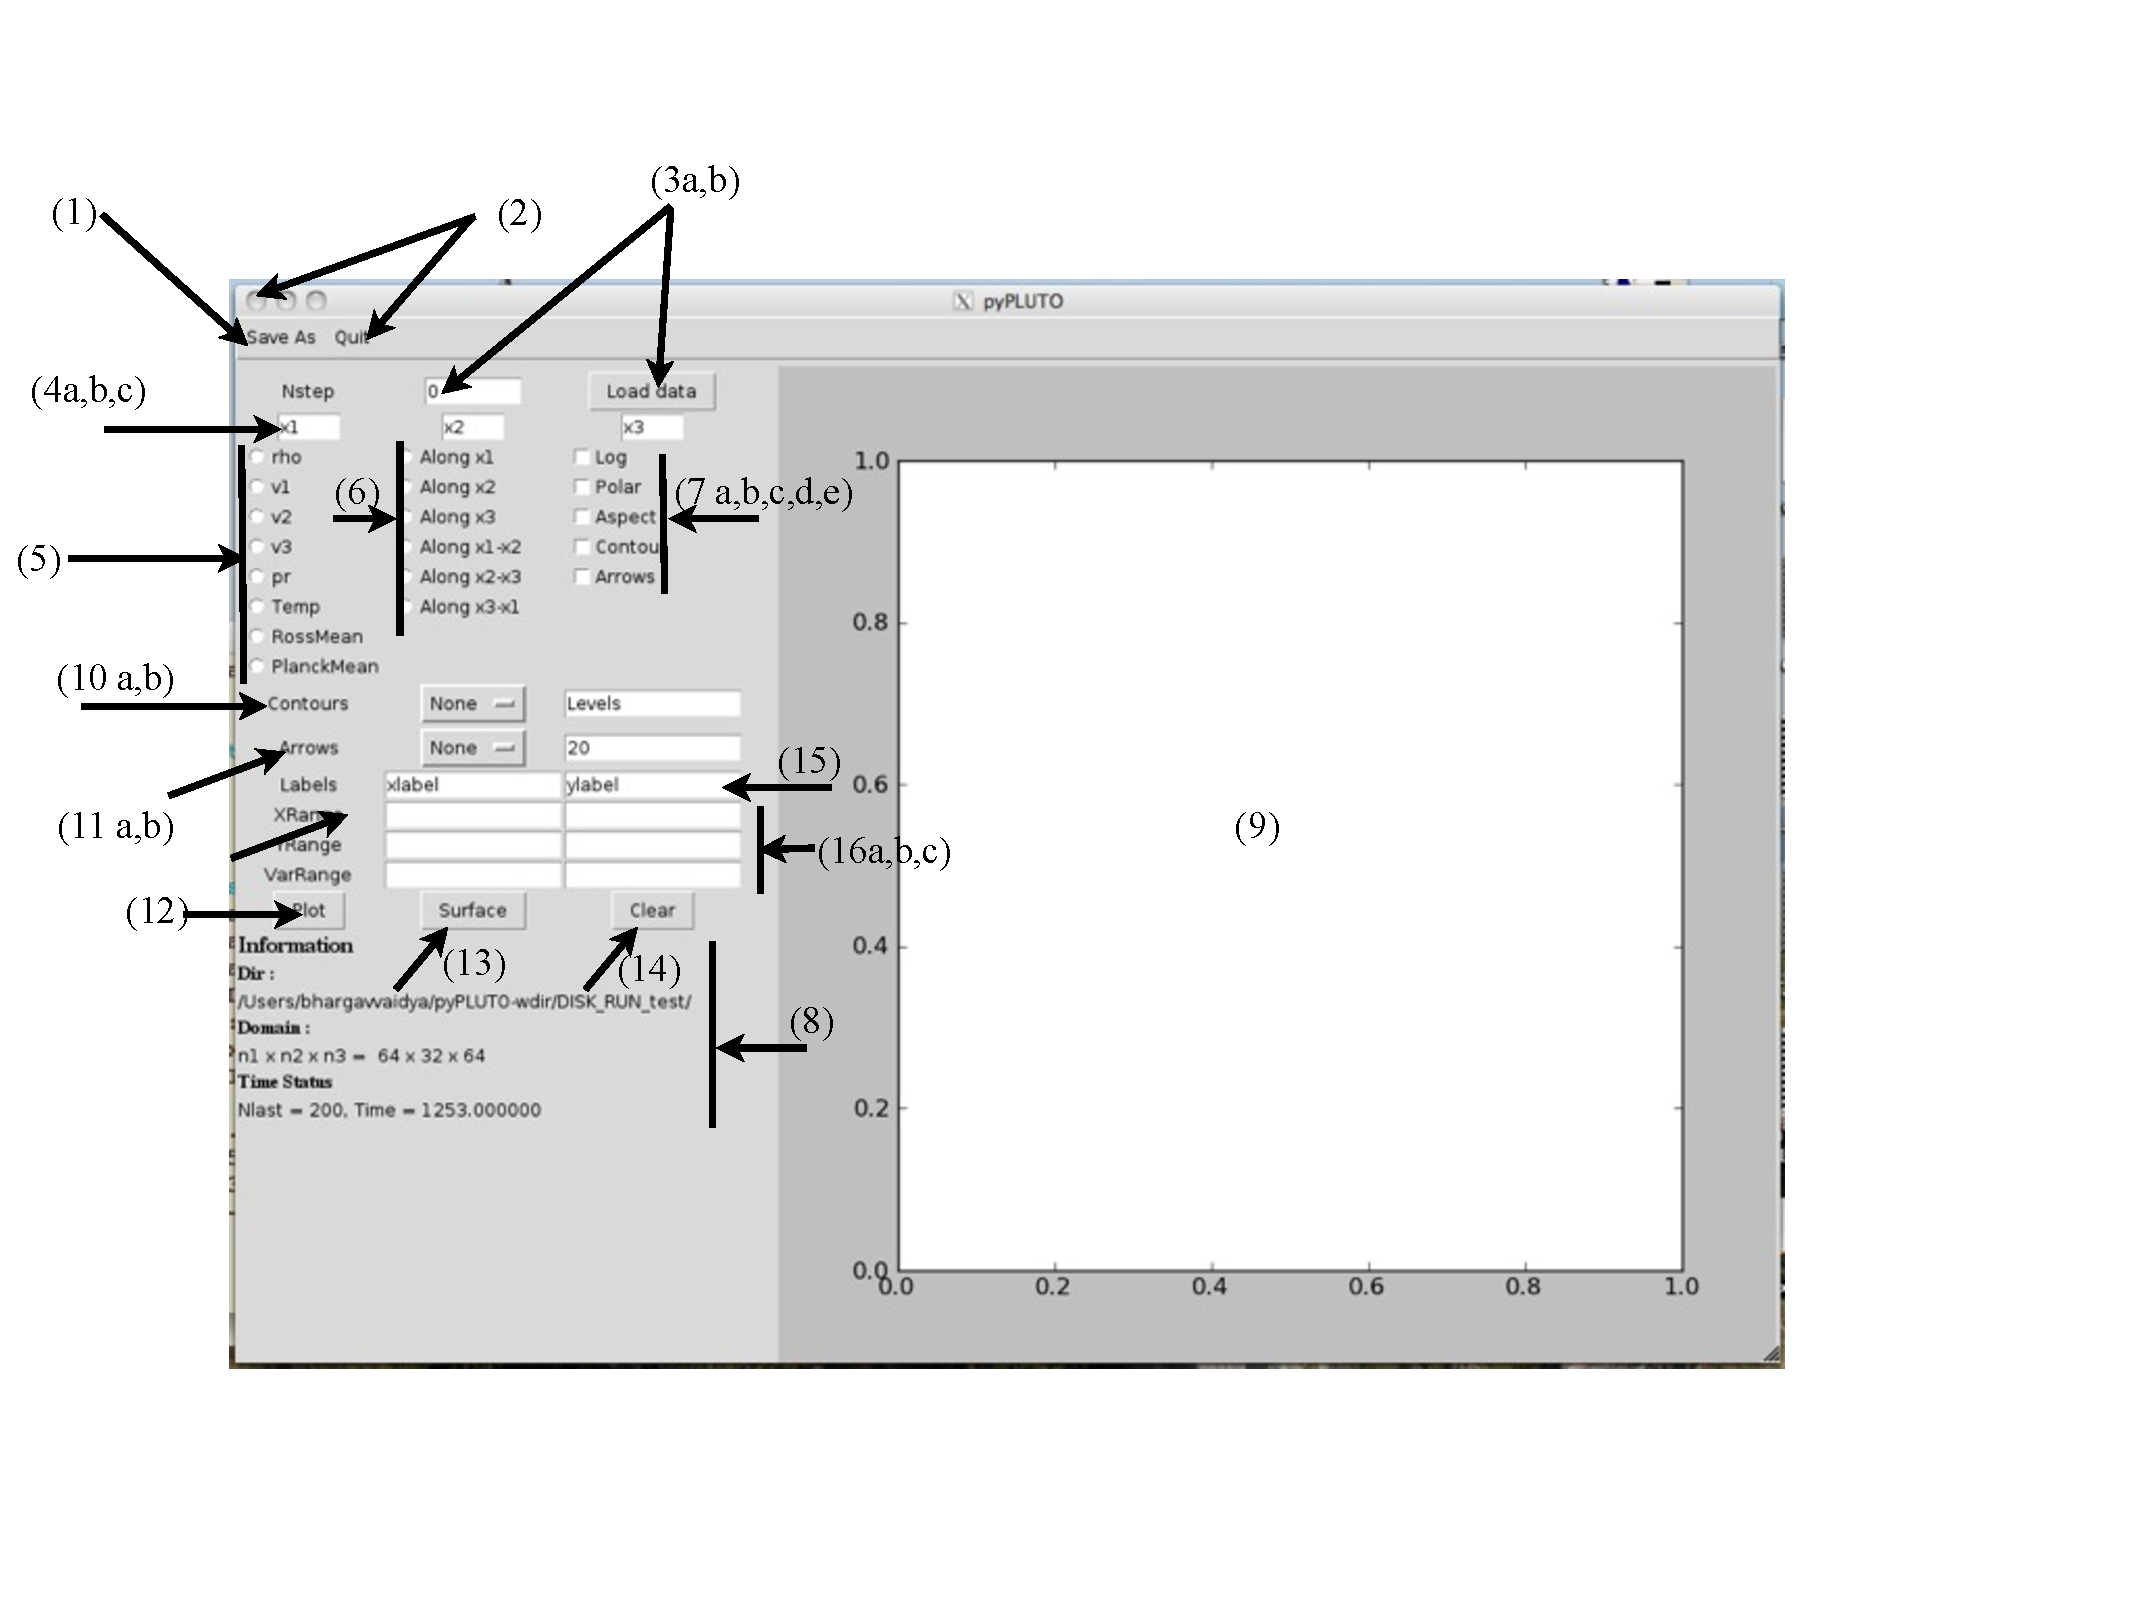
\includegraphics{GetStarted.pdf}
\end{figure}

The Graphic User Interface of the pyPLUTO code for a typical
three dimensional Hydrodynamical example. The various functionality
are marked with numbers as shown in the figure. In-detailed
description of these functionalities are described below.

The various functionalities in the Graphic User Interface (GUI) of the
pyPLUTO code are explained in details below:

1. \emph{Save As} : The drop down menu allows the user to save the figure
displayed in various
formats viz. `eps', `pdf', `jpg', `png'.

2. \emph{Quit} : The user can close the GUI using this
button.

3. \emph{Loading the Data} :  This allows the user to load
data.
\begin{quote}

a. \emph{Nstep} : The number of the data file should be inputted in the
blank panel provided. By default initial data file i.e. Nstep = 0 is
loaded. The input number should be a valid positive number and the
corresponding data file should exists in the working directory.

b. \emph{Load Data} : The user can click on this button to load the
appropriate data file whose number is inputted in the Nstep
panel. Each time the user modifies the value in the Nstep field, this
button needs to be clicked to load the corresponding file.
\end{quote}

4. \emph{Axis cuts} : The user can choose the appropriate values in these
panels to plot/image a particular cut/slice.
No default value is set so error will occur if invalid entry is inputted.
\begin{quote}

a. \emph{x1} : The field to input the x1 cut value. This field should not be
blank if the user either chooses \emph{Along x2} or \emph{Along x3} or \emph{Along
x2-x3} in (6). This field is disabled if the problem considered is
1-D.

b. \emph{x2} : The field to input the x2 cut value. This field should not
be blank if the user either chooses \emph{Along x1} or \emph{Along x3} or
\emph{Along x3-x1} in (6). This field is disabled if the
problem considered is 1-D.

c. \emph{x3} : The field to input the x3 cut value. This field should not
be blank if the user either chooses \emph{Along x1} or \emph{Along x2} or
\emph{Along x1-x2} in (6).  This field is disabled if the
problem considered is either 1-D or 2-D.
\end{quote}

5. \emph{Choose Variables} : The user can choose the variable to plot from the list. This list also includes any additional variable stored using the \emph{userdef\_output.c}. So basically all the variables
listed in the \emph{dbl.out} are enlisted in this column. The code will
have a disabled \emph{Plot} and  \emph{Surface}, until a variable is chosen in this column.

6. \emph{Choose Slices} : The code provides the user to either plot a 1D \emph{Plot} of any of the chosen variable along any axis. Alternatively, the code also allows the user to make a 2D  \emph{Surface} image along
any combination of two axes. This column is redundant in case the
numerical problem under consideration is a 1D problem. With the choice
of the slice, the user should also have appropriate axis cuts
specified as mentioned above else the code will result into an error.

7. \emph{Additional Processing} : The GUI interface allows the user to
carry some additional processing on the variable chosen. They are the
following -
\begin{quote}

a. \emph{Log} : The user can plot logarithmic values using this
option.

b. \emph{Polar} : The user can use this option to project the data from
Spherical coordinates to Cylindrical coordinates. In the present
version, the code handles the projection in the r-\(\theta\) plane
(Along x1-x2) and the r-\(\phi\) plane (Along x3-x1).

c. \emph{Aspect} : Choosing this option allows the user to ensure that the
image (only the Surface) produced has proper aspect ratio. By default
the aspect ratio is set to `auto'.

d. \emph{Contour} : The user can choose this option to overplot the
surface
plot with contours {[}see (10 a,b){]}.

e. \emph{Arrow} : The user can choose this option to overplot the surface
plot with vector arrows {[}see (11 a,b){]}.
\end{quote}

8. \emph{Information Panel} : The user can view the basic information
regarding the problem under consideration. In this panel, the user
can get information of the current working directory, along with the
domain of the numerical problem and finally also the final time
step of that problem.

9. \emph{Figure Window} : In this panel the corresponding \emph{Plot} or the \emph{Surface} (image with colorbar) will be displayed. In
order that the GUI fits into the whole screen, the user can play with
the size of the figure by modifying the code and specifying the size
of the figure window. The default value is : figsize=(7,7).

10. \emph{Contours} : The user can activate this option by choosing the
\emph{Contour} tab {[}7(d){]}.
\begin{quote}

a. \emph{Contour Variable} : The 2D contours of listed variables can be plotted on
the surface plot. The user can choose among all the variables
that are available for plotting along with additional provision
{[}only for the MHD problem{]} of plotting the \emph{Current}
{[}x1*b3{]} and \emph{Magnetic field lines} {[}x1*A3{]}. The Magnetic
field lines contour will only work if the code data consists
information on the vector potential `A3'.
The list by default is set to `None' and thus
will give error is the user tries to plot contours without
choosing the appropriate variable from the drop down list.

b. \emph{Contour Levels} : The user can provide the contours levels which is required separated by `,'. If the user does not
wish to provide the levels then by default a total of 5 contours of automatically chosen levels will be displayed. Further, the
user can also choose to display logarithmic contours by having the
first entry in this panels as \emph{log}. For example,
\begin{itemize}
\item {} 
log,-1.5,-1.8,-2.0 : This plots the logarithmic contours for the chosen Contour variable at levels marked by 10\textasciicircum{}\{-1.5\}, 10\textasciicircum{}\{-1.8\} and 10\textasciicircum{}\{-2.0\}

\item {} 
1.0,2.0,3.0 : This will display normal contours for the chosen Contour variable at levels marked by 1.0, 2.0, and 3.0

\item {} 
Blank {[}Default{]}: 5 contours of automatically chosen  levels will be displayed

\end{itemize}

There is no limit to the number of levels that can be inputed in this
field. By convention all negative contours will be shown as
\emph{dashes}. Incase of logarithmic contours, the \emph{dashes} would
represent contours for levels less than unity.
\end{quote}

11. \emph{Arrows} : The user can activate this option by choosing the
`Arrows' tab {[}7(e){]}.
\begin{quote}

a. \emph{Arrow Variable} : The vector arrows of velocity field {[}Vp and
Vp\_norm{]} and the magnetic field {[}Bp and Bp\_norm{]} (only in
MHD) can be displayed. The options of . The variables with `\_norm' indicate that the
arrows are normalized, i.e. each arrow will have unit length.
The list by default is set to `None' and thus
will give error is the user tries to plot arrows without
choosing the appropriate variable from the drop down list.

b. \emph{Arrow Spacing} : The user can provide the spacing
value which indicates the size of the congrid matrix used to
create the vector plots. Higher values will produce a more
``dense'' plot. Default is set to 20.
\end{quote}

12. \emph{Plot} : This button is by default deactivated and it will be active only when the user has fulfilled the conditions of valid
loading of data {[}(3) a,b{]}, choosing the variable {[}(5){]} and choosing to
plot either Along x1 or Along x2 or Along x3 {[}(6){]}.  Only in case of
1-D numerical problems this button will be activated by default.

13. \emph{Surface} : This button is by default deactivated and it will be
active only when the user has fulfilled the conditions of valid
loading of data {[}(3) a,b{]}, choosing the variable {[}(5){]} and choosing to
plot either Along x1-x2 or Along x2-x3 or Along x3-x1
{[}(6){]}. Consecutively pressing this button will clear the existing
image and create a new one.

14. \emph{Clear} : This button allows the user to
clear the plot.

15. \emph{Labels} : The user can choose the x and y labels for
their plots/images. The user can also use standard TeX symbols within
the `\$' sign. By default they are set to `xlabel' and `ylabel' respectively.

16. \emph{Ranges} : The user can choose range of values to be displayed
from these panels.
\begin{quote}

a. \emph{Xrange} : To set the minimum (left entry) and maximum (right
entry) range of the X axis. A `blank' entry would mean that by
default the minimum and the maximum of the X vector will be shown (i.e. the full range).

b. \emph{Yrange} : To set the minimum (left entry) and maximum (right
entry) range of the Y axis. A `blank' entry would mean that by default the minimum and the maximum of the Y
vector will be shown (i.e. the full range). This becomes
ineffective in case if the user wants to plots a line. To set the
range for the Y axis in case of `Plot', the user should use the
VarRange option.

c. \emph{VarRange} : To set the minimum (left entry) and maximum
(right entry) range of the Variable. A `blank' entry
would mean that by default the minimum and the maximum of the Variable
will be shown (i.e. the full range). In case the user wants a
`Surface' image then with this option the user can choose the
maximum and the minimum of the image. In case of `Plot', this
becomes the Y axis range.
\end{quote}


\chapter{Indices and tables}
\label{index:indices-and-tables}\begin{itemize}
\item {} 
\emph{genindex}

\item {} 
\emph{search}

\end{itemize}


\renewcommand{\indexname}{Python Module Index}
\begin{theindex}
\def\bigletter#1{{\Large\sffamily#1}\nopagebreak\vspace{1mm}}
\bigletter{p}
\item {\texttt{pyPLUTO}}, \pageref{index:module-pyPLUTO}
\end{theindex}

\renewcommand{\indexname}{Index}
\printindex
\end{document}
